\documentclass[a4paper]{article}
%\documentclass[a4paper, twocolumn]{article}

% Options possibles : 10pt, 11pt, 12pt (taille de la fonte)
%                     oneside, twoside (recto simple, recto-verso)
%                     draft, final (stade de développement)
%\usepackage{graphicx}
\usepackage[pdftex]{graphicx}
\usepackage[utf8]{inputenc}
\usepackage[T1]{fontenc}
\usepackage[francais]{babel} 
\usepackage{fancyhdr}

\usepackage[a4paper]{geometry}
\usepackage{subfig}

\title{Calcul de couture minimale \\ {\large ESIR3 -- Imagerie Numérique -- CAV}}         
\author{Maxime \textsc{Broy} \and Florent \textsc{Guiotte}}
%\date{}                   
\pagestyle{fancy}

%\sloppy
\begin{document}
\maketitle 
\begin{abstract}
L'objectif initial du projet était l'implémentation du papier Scene Completion Using Millions of Photographs [Hays et Efros. 2007]. 
Ce dernier consiste à remplacer dans une image toute une région par une scène présente dans une autre image provenant d'une collection de photographies. 
L'algorithme explore cette collection jusqu'à trouver une image avec une sémantique correspondante sans couture.
On cherche donc à remplacer une région de l'image cible par quelque chose de <<plausible>>. 
Il s'agit d'une technique difficilement quantifiable puisque le résultat repose sur la perception visuelle humaine. 
En pratique, ce projet s'est concentré sur une des briques de cette algorithme~: 
le calcul de la couture minimale entourant l'objet que l'on veut transférer d'une image à une autre. 
\end{abstract}

\tableofcontents

\section{Introduction et concept}               % Commencer une section, etc.

\begin{figure}[!ht]%htp]
    \centering
    \subfloat[image cible]{\label{pres:bg}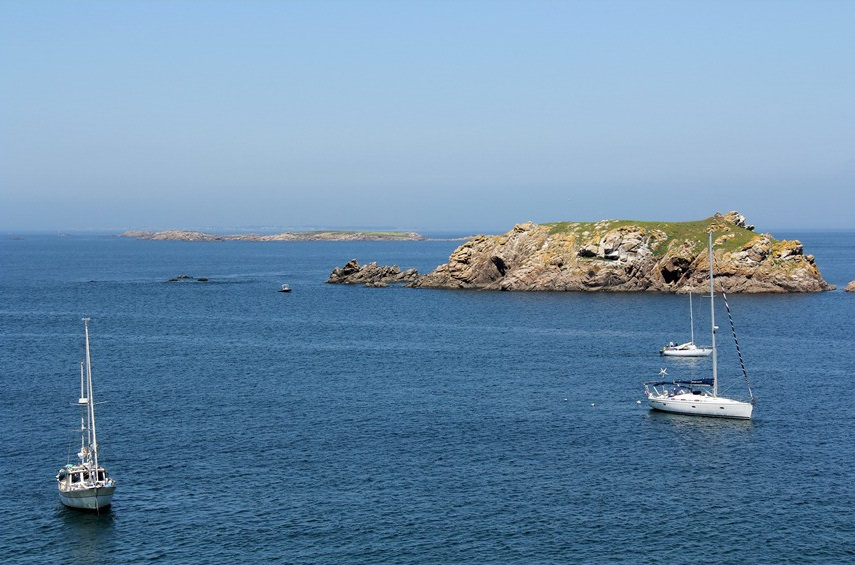
\includegraphics[width=0.48\textwidth]{img/bg.jpg}}
    \hspace{0.030\textwidth}
    \subfloat[image source]{\label{pres:fg}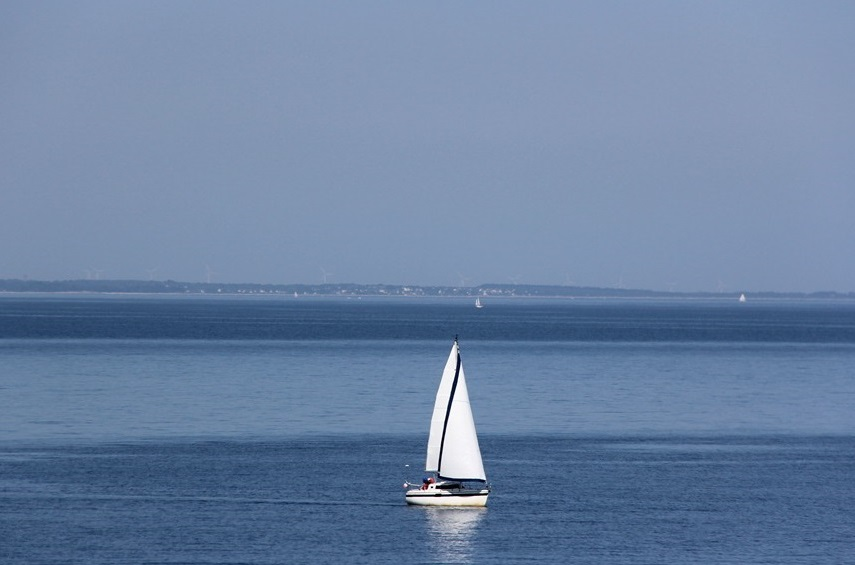
\includegraphics[width=0.48\textwidth]{img/fg.jpg}}
    \caption{Les images de la démonstration}
    \label{pres}
\end{figure}

L'idée est de <<découper>> une région dans l'image source, ici le voilier de la figure \ref{pres:fg} page
\pageref{pres:fg}, pour la transposer dans l'image cible figure \ref{pres:bg}. 
Le voilier devra alors s'intégrer le plus parfaitement possible dans son environnement. L'idée est donc de
calculer quels sont les pixels entourant le voilier que nous allons transposer avec lui dans l'image cible.

\section{Méthode}         
Notre méthode consiste à obtenir un masque de l'image source (figure \ref{gc:mask}) en utilisant la fonction GrabCut d'OpenCV. 
Ensuite, nous calculons l'énergie entre les deux images. C'est en utilisant le masque en sortie du GrabCut et l'énergie que nous 
pouvons ensuite calculer les cartes d'énergie cumulée. La couture qui minimise cette énergie cumulée sera celle retenue.

\subsection{Grabcut}      
On utilise la fonction GrabCut d'Open CV.
\begin{figure}[!ht]%htp]
    \centering
    \subfloat[image source]{\label{gc:fg}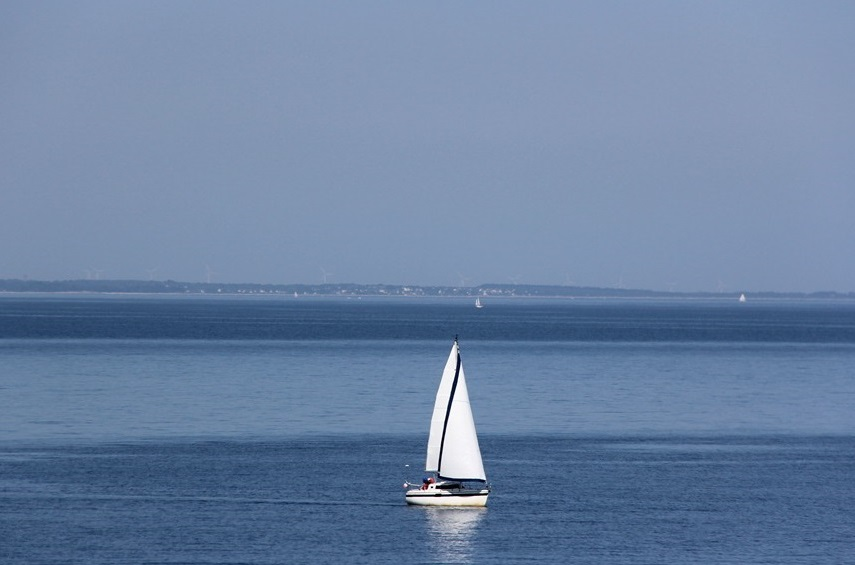
\includegraphics[width=0.48\textwidth]{img/fg.jpg}}
    \hspace{0.030\textwidth}
    \subfloat[masque]{\label{gc:mask}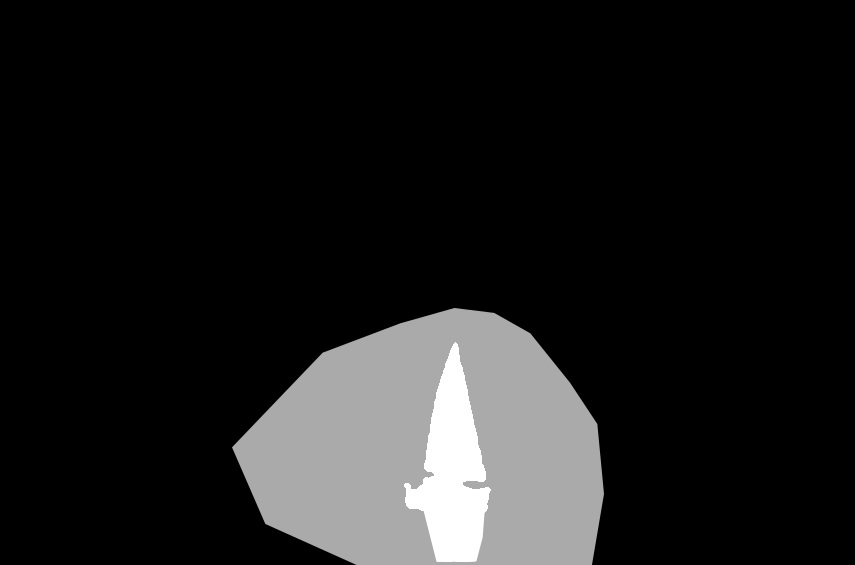
\includegraphics[width=0.48\textwidth]{img/mask.jpg}}
    \caption{Utilisation du GrabCut pour déterminer automatiquement un masque}
    \label{gc}
\end{figure}

L'algorithme du grabcut permet d'extraire le fond d'une image. 
Nous avons utilisé cet algorithme pour créer semi automatiquement le masque que nous utiliserons plus tard
pour déterminer le chemin de la couture minimum. 
Ce masque (figure \ref{gc:mask}) contient trois valeurs différentes~:

\begin{itemize}
    \item Le fond (noir), déterminé par l'utilisateur. 
    \item Le sujet (blanc), détouré par l'algorithme du grabcut selon les entrées de l'utilisateur.
    \item La marge (gris), correspond à la zone entre le fond et le sujet, ayant une probabilité d'appartenir au fond. C'est dans cette zone que nous allons chercher la couture minimale.
\end{itemize}

\subsection{Calcul d'énergie}

Nous avons essayé plusieurs techniques de calcul d'énergie~:

\begin{itemize}
    \item La différence au carrée entre les deux images
    \item La norme du Sobel en RBG entre les deux images
    \item La norme du Sobel en LAB entre les deux images
\end{itemize}

Pour cet article nous avons retenu la différence au carré et le sobel en LAB. Le sobel RGB présente des résultats
similaires au sobel LAB, la faute à nos images choisies pour les démonstrations. % TODO: formulation
Les résultats de ces calculs sont visibles sous forme de cartes d'énergie figure \ref{energie}.

\begin{figure}[!ht]%htp]
    \centering
    \subfloat[Valeur absolue de la différence au carré]{\label{energie:e}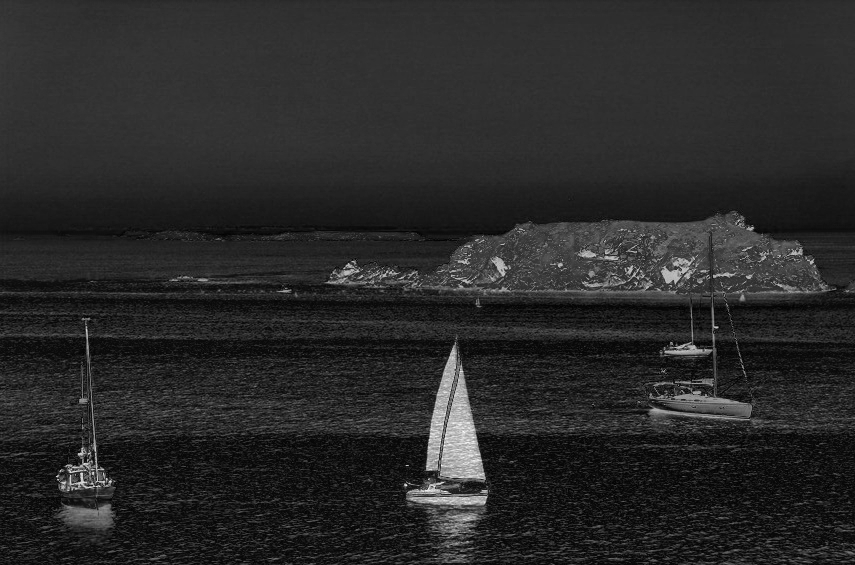
\includegraphics[width=0.48\textwidth]{img/energy.png}}
    \hspace{0.030\textwidth}
    \subfloat[Sobel]{\label{energie:sobel}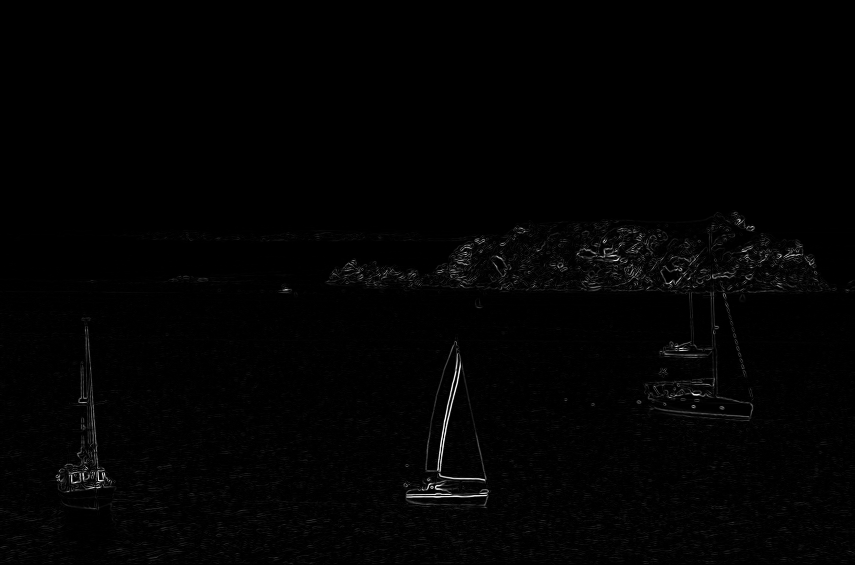
\includegraphics[width=0.48\textwidth]{img/energy_sobel.png}}
    \caption{Cartes d'énergie}
    \label{energie}
\end{figure}

\subsection{Calcul des cartes d'énergie cumulée}

Tout d'abord, il faut définir une ligne de pixels partant du bord du masque de fond jusqu'au masque du sujet (on appellera
cette ligne {\em steam}, pour {\em start seam}). %Il s'agit de la ligne rouge sur la figure \ref{derp}.
Cette ligne est choisie automatiquement pour être la plus courte possible à travers la marge.

Les raisons pour garder cette ligne la plus courte possible sont multiples. D'une part, les coutures minimales
vont toutes passer par ce <<goulot d'étranglement>>. D'autre part, notre méthode génère une carte d'énergie
cumulée par pixel composant cette ligne de départ. Afin de minimiser le temps d'éxecution de l'algorithme il
est judicieux de limiter au maximum ces calculs.

Une carte d’énergie cumulée correspond à la somme de l'énergie de chaque pixel de la carte d'énergie. 
On part d’un pixel de steam jusqu’à faire le tour de l’objet en explorant le voisinage à l'aide d'une connexité 8.
Plusieurs techniques ont été testée pour le cumul de l'énergie. Pour favoriser les bons résultats on propage
en priorité le calcul de l'énergie parmis les voisins des pixels les plus prometteurs (ayant une énergie moins élevés) 
avec le risque de faire apparaitre des minimums locaux.

Un exemple de ces cartes d'énergie cumulées selon les deux cartes d'énergies précédemment calculées, soit la
valeur absolue de la différence au carré et sobel, sont visibles figure \ref{ecum}. Ces exemples sont
respectivement l'une des carte d'énergie cumulées parmis toutes celles calculées, pour chaque pixel composant la ligne de départ.

\begin{figure}[!ht]%htp]
    \centering
    \subfloat[Valeur absolue de la différence au carré]{\label{ecum:e}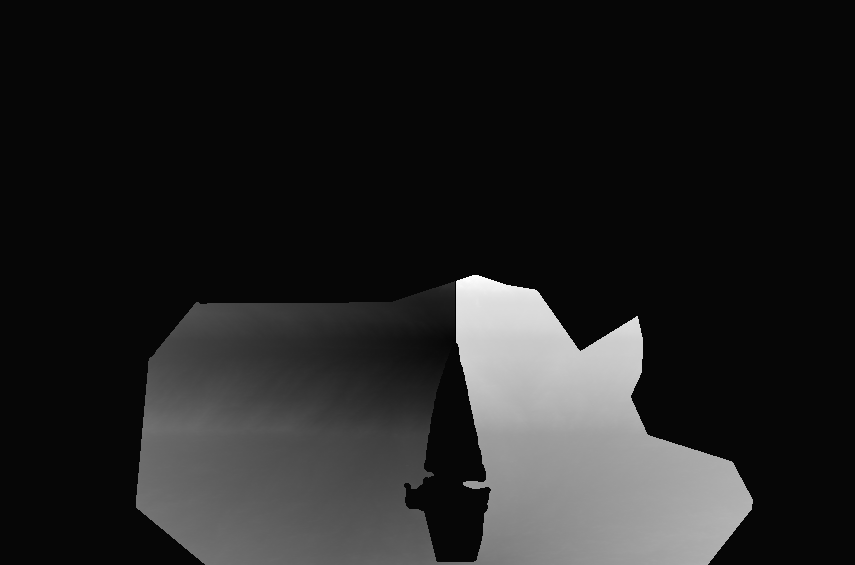
\includegraphics[width=0.48\textwidth]{img/energy_cum.png}}
    \hspace{0.030\textwidth}
    \subfloat[Sobel]{\label{ecum:sobel}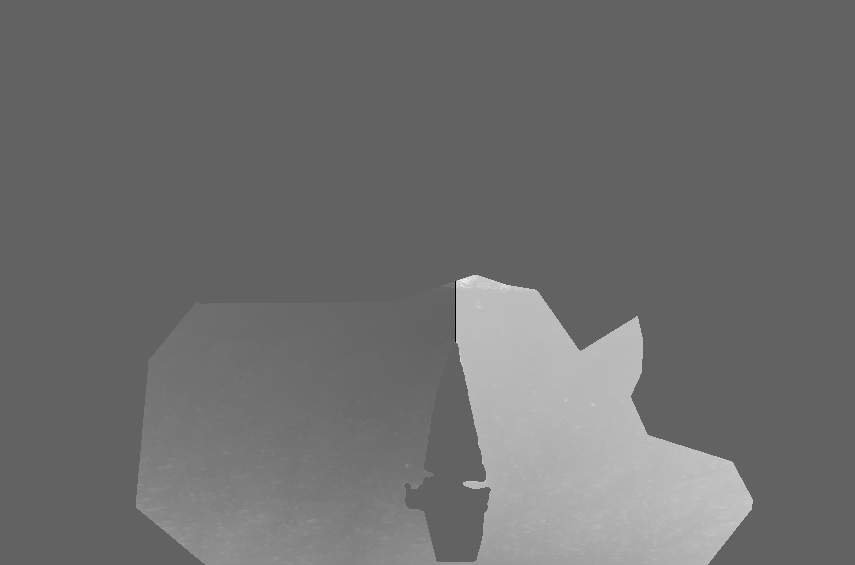
\includegraphics[width=0.48\textwidth]{img/energy_cum_sobel.png}}
    \caption{Cartes d'énergie cumulée}
    \label{ecum}
\end{figure}

\subsection{Calcul de la couture}

\begin{figure}[!ht]%htp]
    \centering
    \subfloat[Valeur absolue de la différence au carré]{\label{allseams:e}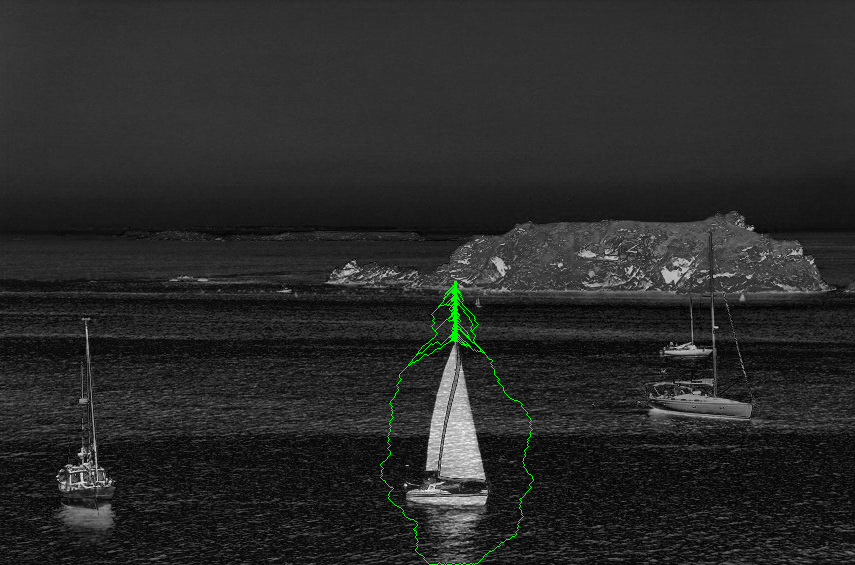
\includegraphics[width=0.48\textwidth]{img/all_seams.png}}
    \hspace{0.030\textwidth}
    \subfloat[Sobel]{\label{allseams:sobel}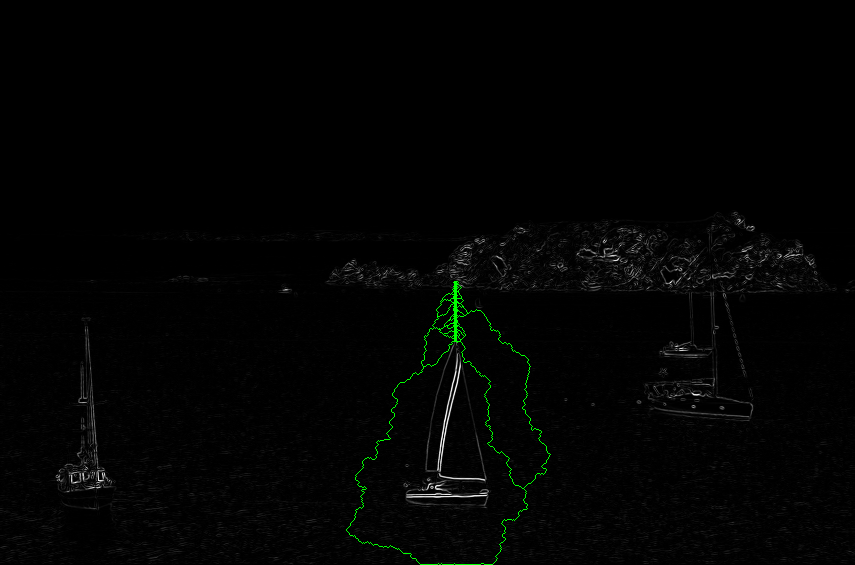
\includegraphics[width=0.48\textwidth]{img/all_seam_sobel.png}}
    \caption{Coutures minimisant l'énergie, affichées sur carte d'énergie}
    \label{allseams}
\end{figure}

\begin{figure}[!ht]%htp]
    \centering
    \subfloat[Valeur absolue de la différence au carré]{\label{bestseam:e}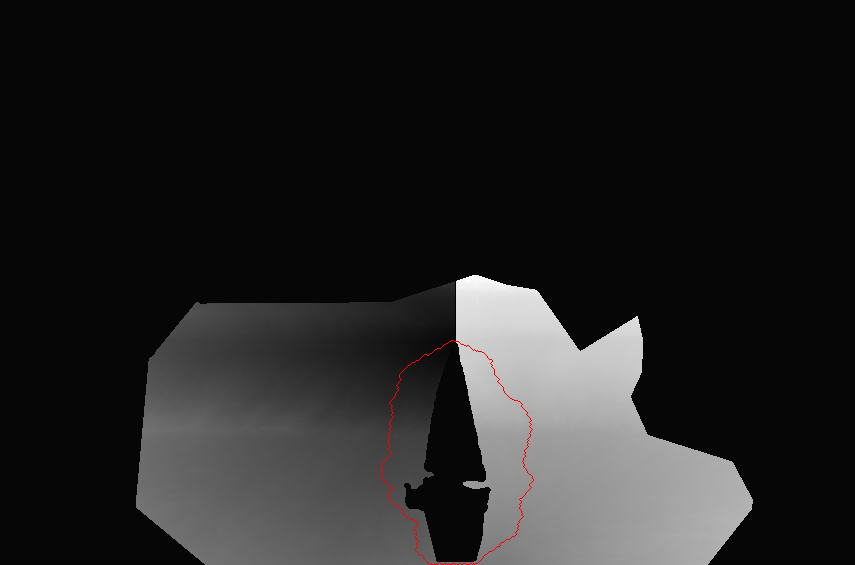
\includegraphics[width=0.48\textwidth]{img/min_seam.png}}
    \hspace{0.030\textwidth}
    \subfloat[Sobel]{\label{bestseam:sobel}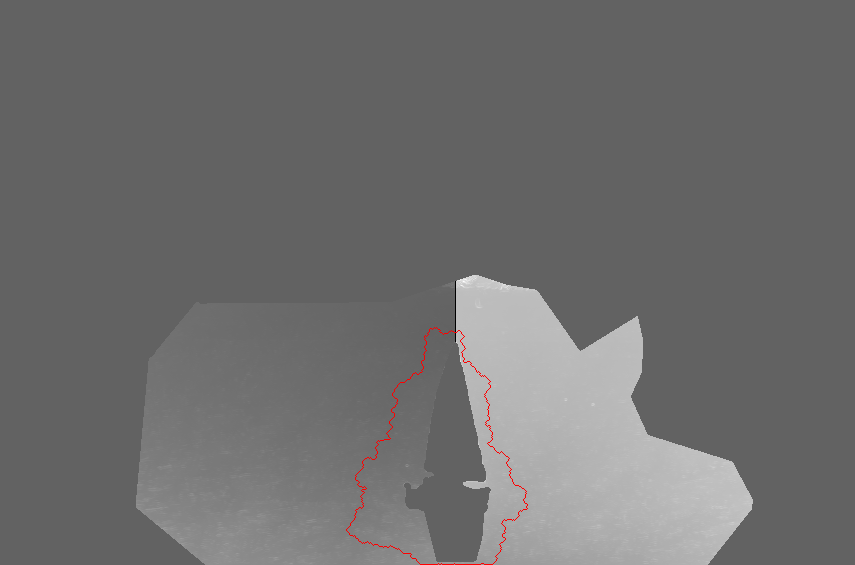
\includegraphics[width=0.48\textwidth]{img/min_seam_sobel.png}}
    \caption{Meilleure des coutures, affichée sur carte d'énergie cumulée}
    \label{bestseam}
\end{figure}
Pour chaque pixel qui n’est pas noir et qui n’est pas déjà visité, on explore ses voisins en sélectionnant celui dont l’énergie correspondante (dans la carte d’énergie) est minimale. Cela jusqu'à avoir atteint le point d'arrivée (voisin de droite du point de départ).

\section{Résultat}

Quisque dolor odio, aliquam quis, placerat sed, hendrerit eu, magna. Cras at
turpis et mi imperdiet lobortis. Nam eu massa et eros congue gravida. Sed
luctus. Nullam sit amet nunc a tellus lacinia tempor. Praesent tincidunt ligula
quis lacus. Nullam sodales, mi sed venenatis egestas, risus turpis dictum elit,
ac egestas augue eros eget erat. Cras faucibus.

\begin{figure}[!ht]%htp]
    \centering
    \subfloat[Valeur absolue de la différence au carré]{\label{results:e}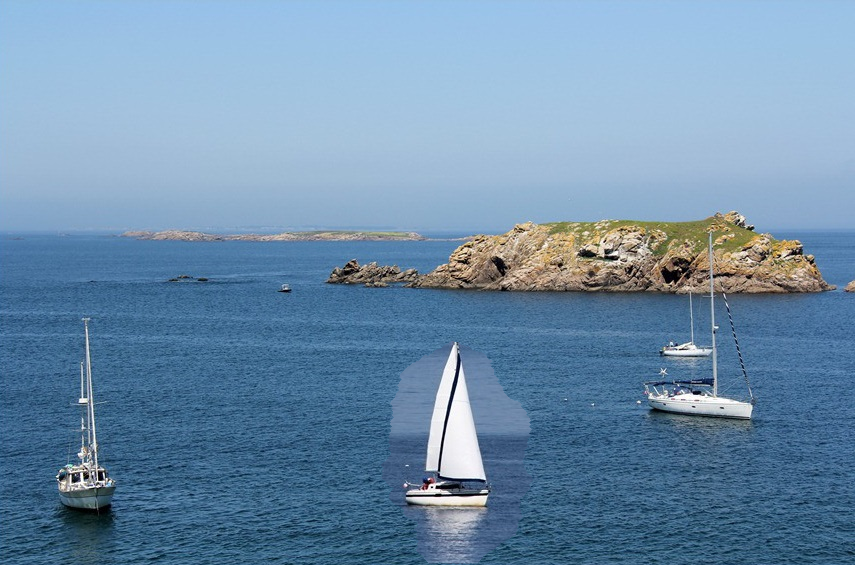
\includegraphics[width=0.48\textwidth]{img/result.png}}
    \hspace{0.030\textwidth}
    \subfloat[Sobel]{\label{results:sobel}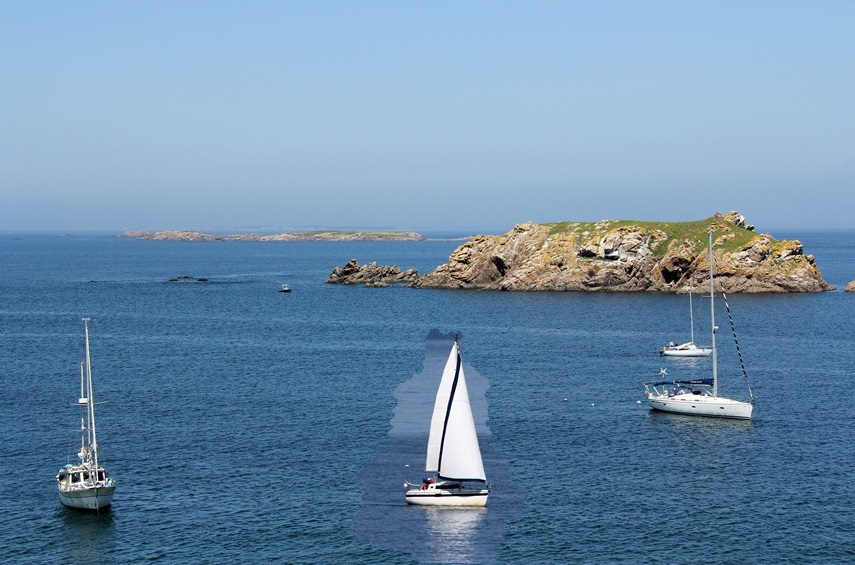
\includegraphics[width=0.48\textwidth]{img/result_sobel.png}}
    \caption{Fusion des deux images suivant la couture minimale}
    \label{results}
\end{figure}

\section{Performance}

Quisque dolor odio, aliquam quis, placerat sed, hendrerit eu, magna. Cras at
turpis et mi imperdiet lobortis. Nam eu massa et eros congue gravida. Sed
luctus. Nullam sit amet nunc a tellus lacinia tempor. Praesent tincidunt ligula
quis lacus. Nullam sodales, mi sed venenatis egestas, risus turpis dictum elit,
ac egestas augue eros eget erat. Cras faucibus.

\section{Références}

[1] J. Hays and A. A. Efros.  2007. Scene completion using millions of photographs. ACM Trans. Graph.,
\\

[2] JIA, J., SUN, J., TANG, C.-K., AND SHUM, H.-Y. 2006. Drag and-drop pasting. ACM Trans. Graph.,



\end{document}
